%%%%%%%%%%%%%%%%%%%%%%%%%%%%%%%%%%%%%%%%
% datoteka diploma-FRI-vzorec.tex
%
%POZOR: ta verzija ne producira pdf datoteke v pdf/A formatu!!!
%namenjena je le za nalogo pri Diplomskem seminarju!
%
% vzorčna datoteka za pisanje diplomskega dela v formatu LaTeX
% na UL Fakulteti za računalništvo in informatiko
%
% na osnovi starejših verzij vkup spravil Franc Solina, maj 2021
% prvo verzijo je leta 2010 pripravil Gašper Fijavž
%
% za upravljanje z literaturo ta vezija uporablja BibLaTeX
%
% svetujemo uporabo Overleaf.com - na tej spletni implementaciji LaTeXa ta vzorec zagotovo pravilno deluje
%

\documentclass[a4paper,12pt,openright]{book}
%\documentclass[a4paper, 12pt, openright, draft]{book}  Nalogo preverite tudi z opcijo draft, ki pokaže, katere vrstice so predolge! Pozor, v draft opciji, se slike ne pokažejo!
 
\usepackage[utf8]{inputenc}   % omogoča uporabo slovenskih črk kodiranih v formatu UTF-8
\usepackage[slovene,english]{babel}    % naloži, med drugim, slovenske delilne vzorce
\usepackage[pdftex]{graphicx}  % omogoča vlaganje slik različnih formatov
\usepackage{fancyhdr}          % poskrbi, na primer, za glave strani
\usepackage{amssymb}           % dodatni matematični simboli
\usepackage{amsmath}           % eqref, npr.
\usepackage{hyperxmp}
\usepackage[hyphens]{url}
\usepackage{csquotes}
\usepackage[pdftex, colorlinks=true,
						citecolor=black, filecolor=black, 
						linkcolor=black, urlcolor=black,
						pdfproducer={LaTeX}, pdfcreator={LaTeX}]{hyperref}

\usepackage{color}
\usepackage{float}
\usepackage{soul}
\usepackage{listings}
\usepackage[
backend=biber,
style=numeric,
sorting=nty,
]{biblatex}


\addbibresource{literatura.bib} %Imports bibliography file


%%%%%%%%%%%%%%%%%%%%%%%%%%%%%%%%%%%%%%%%
%	DIPLOMA INFO
%%%%%%%%%%%%%%%%%%%%%%%%%%%%%%%%%%%%%%%%
\newcommand{\ttitle}{Upravljanje z identitetami}
\newcommand{\ttitleEn}{Diploma thesis template}
\newcommand{\tsubject}{\ttitle}
\newcommand{\tsubjectEn}{\ttitleEn}
\newcommand{\tauthor}{David Konc}
\newcommand{\tkeywords}{računalnik, identitete, upravljanje, varnost}
\newcommand{\tkeywordsEn}{computer, identity, management, security}

%%%%%%%%%%%%%%%%%%%%%%%%%%%%%%%%%%%%%%%%
%	HYPERREF SETUP
%%%%%%%%%%%%%%%%%%%%%%%%%%%%%%%%%%%%%%%%
\hypersetup{pdftitle={\ttitle}}
\hypersetup{pdfsubject=\ttitleEn}
\hypersetup{pdfauthor={\tauthor}}
\hypersetup{pdfkeywords=\tkeywordsEn}

%%%%%%%%%%%%%%%%%%%%%%%%%%%%%%%%%%%%%%%%
% postavitev strani
%%%%%%%%%%%%%%%%%%%%%%%%%%%%%%%%%%%%%%%%  

\addtolength{\marginparwidth}{-20pt} % robovi za tisk
\addtolength{\oddsidemargin}{40pt}
\addtolength{\evensidemargin}{-40pt}

\renewcommand{\baselinestretch}{1.3} % ustrezen razmik med vrsticami
\setlength{\headheight}{15pt}        % potreben prostor na vrhu
\renewcommand{\chaptermark}[1]%
{\markboth{\MakeUppercase{\thechapter.\ #1}}{}} \renewcommand{\sectionmark}[1]%
{\markright{\MakeUppercase{\thesection.\ #1}}} \renewcommand{\headrulewidth}{0.5pt} \renewcommand{\footrulewidth}{0pt}
\fancyhf{}
\fancyhead[LE,RO]{\sl \thepage} 
%\fancyhead[LO]{\sl \rightmark} \fancyhead[RE]{\sl \leftmark}
\fancyhead[RE]{\sc \tauthor}              % dodal Solina
\fancyhead[LO]{\sc Diplomska naloga}     % dodal Solina


\newcommand{\BibLaTeX}{{\sc Bib}\LaTeX}
\newcommand{\BibTeX}{{\sc Bib}\TeX}

%%%%%%%%%%%%%%%%%%%%%%%%%%%%%%%%%%%%%%%%
% naslovi
%%%%%%%%%%%%%%%%%%%%%%%%%%%%%%%%%%%%%%%%  

\newcommand{\autfont}{\Large}
\newcommand{\titfont}{\LARGE\bf}
\newcommand{\clearemptydoublepage}{\newpage{\pagestyle{empty}\cleardoublepage}}
\setcounter{tocdepth}{1}	      % globina kazala

%%%%%%%%%%%%%%%%%%%%%%%%%%%%%%%%%%%%%%%%
% konstrukti
%%%%%%%%%%%%%%%%%%%%%%%%%%%%%%%%%%%%%%%%  
\newtheorem{izrek}{Izrek}[chapter]
\newtheorem{trditev}{Trditev}[izrek]
\newenvironment{dokaz}{\emph{Dokaz.}\ }{\hspace{\fill}{$\Box$}}


%%%%%%%%%%%%%%%%%%%%%%%%%%%%%%%%%%%%%%%%%%%%%%%%%%%%%%%%%%%%%%%%%%%%%%%%%%%%%%%
%% PDF-A
%%%%%%%%%%%%%%%%%%%%%%%%%%%%%%%%%%%%%%%%%%%%%%%%%%%%%%%%%%%%%%%%%%%%%%%%%%%%%%%

%%%%%%%%%%%%%%%%%%%%%%%%%%%%%%%%%%%%%%%% 
% define medatata
%%%%%%%%%%%%%%%%%%%%%%%%%%%%%%%%%%%%%%%% 
\def\Title{\ttitle}
\def\Author{\tauthor, dk2418@student.uni-lj.si}
\def\Subject{\ttitleEn}
\def\Keywords{\tkeywordsEn}

%%%%%%%%%%%%%%%%%%%%%%%%%%%%%%%%%%%%%%%% 
% \convertDate converts D:20080419103507+02'00' to 2008-04-19T10:35:07+02:00
%%%%%%%%%%%%%%%%%%%%%%%%%%%%%%%%%%%%%%%% 
\def\convertDate{%
    \getYear
}

{\catcode`\D=12
 \gdef\getYear D:#1#2#3#4{\edef\xYear{#1#2#3#4}\getMonth}
}
\def\getMonth#1#2{\edef\xMonth{#1#2}\getDay}
\def\getDay#1#2{\edef\xDay{#1#2}\getHour}
\def\getHour#1#2{\edef\xHour{#1#2}\getMin}
\def\getMin#1#2{\edef\xMin{#1#2}\getSec}
\def\getSec#1#2{\edef\xSec{#1#2}\getTZh}
\def\getTZh +#1#2{\edef\xTZh{#1#2}\getTZm}
\def\getTZm '#1#2'{%
    \edef\xTZm{#1#2}%
    \edef\convDate{\xYear-\xMonth-\xDay T\xHour:\xMin:\xSec+\xTZh:\xTZm}%
}

%\expandafter\convertDate\pdfcreationdate 

%%%%%%%%%%%%%%%%%%%%%%%%%%%%%%%%%%%%%%%%
% get pdftex version string
%%%%%%%%%%%%%%%%%%%%%%%%%%%%%%%%%%%%%%%% 
\newcount\countA
\countA=\pdftexversion
\advance \countA by -100
\def\pdftexVersionStr{pdfTeX-1.\the\countA.\pdftexrevision}


%%%%%%%%%%%%%%%%%%%%%%%%%%%%%%%%%%%%%%%%
% XMP data
%%%%%%%%%%%%%%%%%%%%%%%%%%%%%%%%%%%%%%%%  
\usepackage{xmpincl}
%\includexmp{pdfa-1b}

%%%%%%%%%%%%%%%%%%%%%%%%%%%%%%%%%%%%%%%%
% pdfInfo
%%%%%%%%%%%%%%%%%%%%%%%%%%%%%%%%%%%%%%%%  
\pdfinfo{%
    /Title    (\ttitle)
    /Author   (\tauthor, damjan@cvetan.si)
    /Subject  (\ttitleEn)
    /Keywords (\tkeywordsEn)
    /ModDate  (\pdfcreationdate)
    /Trapped  /False
}

%%%%%%%%%%%%%%%%%%%%%%%%%%%%%%%%%%%%%%%%
% znaki za copyright stran
%%%%%%%%%%%%%%%%%%%%%%%%%%%%%%%%%%%%%%%%  

\newcommand{\CcImageCc}[1]{%
	
\includegraphics[scale=#1]{cc_cc_30.pdf}%
}
\newcommand{\CcImageBy}[1]{%
	
\includegraphics[scale=#1]{cc_by_30.pdf}%
}
\newcommand{\CcImageSa}[1]{%
	
\includegraphics[scale=#1]{cc_sa_30.pdf}%
}

%%%%%%%%%%%%%%%%%%%%%%%%%%%%%%%%%%%%%%%%%%%%%%%%%%%%%%%%%%%%%%%%%%%%%%%%%%%%%%%
%%%%%%%%%%%%%%%%%%%%%%%%%%%%%%%%%%%%%%%%%%%%%%%%%%%%%%%%%%%%%%%%%%%%%%%%%%%%%%%

\begin{document}
\selectlanguage{slovene}
\frontmatter
\setcounter{page}{1} %
\renewcommand{\thepage}{}       % preprečimo težave s številkami strani v kazalu

%%%%%%%%%%%%%%%%%%%%%%%%%%%%%%%%%%%%%%%%
%naslovnica
 \thispagestyle{empty}%
   \begin{center}
    {\large\sc Univerza v Ljubljani\\%
%      Fakulteta za elektrotehniko\\% za študijski program Multimedija
%      Fakulteta za upravo\\% za študijski program Upravna informatika
      Fakulteta za računalništvo in informatiko\\%
%      Fakulteta za matematiko in fiziko\\% za študijski program Računalništvo in matematika
     }
    \vskip 10em%
    {\autfont \tauthor\par}%
    {\titfont \ttitle \par}%
    {\vskip 3em \textsc{DIPLOMSKO DELO\\[5mm]         % dodal Solina za ostale študijske programe
%    VISOKOŠOLSKI STROKOVNI ŠTUDIJSKI PROGRAM\\ PRVE STOPNJE\\ RAČUNALNIŠTVO IN INFORMATIKA}\par}%
     UNIVERZITETNI  ŠTUDIJSKI PROGRAM\\ PRVE STOPNJE\\ RAČUNALNIŠTVO IN INFORMATIKA}\par}%
%    INTERDISCIPLINARNI UNIVERZITETNI\\ ŠTUDIJSKI PROGRAM PRVE STOPNJE\\ MULTIMEDIJA}\par}%
%    INTERDISCIPLINARNI UNIVERZITETNI\\ ŠTUDIJSKI PROGRAM PRVE STOPNJE\\ UPRAVNA INFORMATIKA}\par}%
%    INTERDISCIPLINARNI UNIVERZITETNI\\ ŠTUDIJSKI PROGRAM PRVE STOPNJE\\ RAČUNALNIŠTVO IN MATEMATIKA}\par}%
    \vfill\null%
% izberite pravi habilitacijski naziv mentorja!
    {\large \textsc{Mentor}: dr. Andrej Brodnik\par}%
   {\large \textsc{Somentor}:  asist. dr.  Gašper Fele Žorž \par}%
    {\vskip 2em \large Ljubljana, \the\year \par}%
\end{center}
% prazna stran
%\clearemptydoublepage      
% izjava o licencah itd. se izpiše na hrbtni strani naslovnice

%%%%%%%%%%%%%%%%%%%%%%%%%%%%%%%%%%%%%%%%
%copyright stran
%%%%%%%%%%%%%%%%%%%%%%%%%%%%%%%%%%%%%%%%
\newpage
\thispagestyle{empty}

\vspace*{5cm}
{\small \noindent
To delo je ponujeno pod licenco \textit{Creative Commons Priznanje avtorstva-Deljenje pod enakimi pogoji 2.5 Slovenija} (ali novej\v so razli\v cico).
To pomeni, da se tako besedilo, slike, grafi in druge sestavine dela kot tudi rezultati diplomskega dela lahko prosto distribuirajo,
reproducirajo, uporabljajo, priobčujejo javnosti in predelujejo, pod pogojem, da se jasno in vidno navede avtorja in naslov tega
dela in da se v primeru spremembe, preoblikovanja ali uporabe tega dela v svojem delu, lahko distribuira predelava le pod
licenco, ki je enaka tej.
Podrobnosti licence so dostopne na spletni strani \href{http://creativecommons.si}{creativecommons.si} ali na Inštitutu za
intelektualno lastnino, Streliška 1, 1000 Ljubljana.

\vspace*{1cm}
\begin{center}% 0.66 / 0.89 = 0.741573033707865
\CcImageCc{0.741573033707865}\hspace*{1ex}\CcImageBy{1}\hspace*{1ex}\CcImageSa{1}%
\end{center}
}

\vspace*{1cm}
{\small \noindent
Izvorna koda diplomskega dela, njeni rezultati in v ta namen razvita programska oprema je ponujena pod licenco GNU General Public License,
različica 3 (ali novejša). To pomeni, da se lahko prosto distribuira in/ali predeluje pod njenimi pogoji.
Podrobnosti licence so dostopne na spletni strani \url{http://www.gnu.org/licenses/}.
}

\vfill
\begin{center} 
\ \\ \vfill
{\em
Besedilo je oblikovano z urejevalnikom besedil \LaTeX.}
\end{center}

% prazna stran
\clearemptydoublepage

%%%%%%%%%%%%%%%%%%%%%%%%%%%%%%%%%%%%%%%%
% stran 3 med uvodnimi listi
\thispagestyle{empty}
\
\vfill

\bigskip
\noindent\textbf{Kandidat:} David Konc\\
\noindent\textbf{Naslov:} Upravljanje z identitetami\\
% vstavite ustrezen naziv študijskega programa!
\noindent\textbf{Vrsta naloge:} Diplomska naloga na univerzitetnem programu prve stopnje Računalništvo in informatika \\
% izberite pravi habilitacijski naziv mentorja!
\noindent\textbf{Mentor:} dr. Andrej Brodnik\\
\noindent\textbf{Somentor:} asist.dr. Gašper Fele Žorž

\bigskip
\noindent\textbf{Opis:}\\
Doda mentor.

\bigskip
\noindent\textbf{Title:} Naslov diplomskega dela v angleščini

\bigskip
\noindent\textbf{Description:}\\
opis diplome v angleščini

\vfill



\vspace{2cm}

% prazna stran
\clearemptydoublepage

% zahvala
\thispagestyle{empty}\mbox{}\vfill\null\it%
\noindent
Zahvalil bi se družini in prijateljem, ki so mi v času študija stali ob strani ter me podpirali.
Prav tako bi se rad zahvalil mentorju in somentorju za usmerjanje in nasvete ob pisanju diplomskega dela. 
\rm\normalfont

% prazna stran
\clearemptydoublepage

% kazalo
\pagestyle{empty}
\def\thepage{}% preprečimo težave s številkami strani v kazalu
\tableofcontents{}


% prazna stran
\clearemptydoublepage

%%%%%%%%%%%%%%%%%%%%%%%%%%%%%%%%%%%%%%%%
% seznam kratic

\chapter*{Seznam uporabljenih kratic}
Se ne uporabljeno/dokoncano (se vedno samo defaultna stvar) \newline
\noindent\begin{tabular}{p{0.11\textwidth}|p{.39\textwidth}|p{.39\textwidth}}    % po potrebi razširi prvo kolono tabele na račun drugih dveh!
  {\bf kratica} & {\bf angleško}                              & {\bf slovensko} \\ \hline
  {\bf SAML}      & Security Assertion Markup Language               & Označevalni jezik varnostnih trditev \\
  {\bf HTTP} & Hypertext Transfer Protocol & Protokol za prenos hiperteksta \\
%  \dots & \dots & \dots \\
\end{tabular}


% prazna stran
\clearemptydoublepage

%%%%%%%%%%%%%%%%%%%%%%%%%%%%%%%%%%%%%%%%
% povzetek
\addcontentsline{toc}{chapter}{Povzetek}
\chapter*{Povzetek}

\noindent\textbf{Naslov:} \ttitle
\bigskip

\noindent\textbf{Avtor:} \tauthor
\bigskip

%\noindent\textbf{Povzetek:} 
\noindent Leta 2019 sem našel varnostno pomanjkljivost na spletni strani Univerze v Ljubljani, kjer sem opazil pomanjkljivosti pri verifikaciji identitete. V diplomski nalogi zato raziskujem možno rešitev, ki bi ta problem odpravila. Raziskujem prednosti in slabosti vseh ponudnikov za upravljanje identitet v Sloveniji, jih med seboj primerjam ter ponudim možno rešitev. Ugotovitve opravljene raziskave bom predstavil pristojnim na Univerzi v Ljubljani,  s katerimi se bom pogovoril o možnih nadaljnjih postopkih oz. možni implementaciji. 
\bigskip

\noindent\textbf{Ključne besede:} \tkeywords.
% prazna stran
\clearemptydoublepage

%%%%%%%%%%%%%%%%%%%%%%%%%%%%%%%%%%%%%%%%
% abstract
\selectlanguage{english}
\addcontentsline{toc}{chapter}{Abstract}
\chapter*{Abstract}

\noindent\textbf{Title:} \ttitleEn
\bigskip

\noindent\textbf{Author:} \tauthor
\bigskip

%\noindent\textbf{Abstract:} 
\noindent In 2019, I found a security flaw at the University of Ljubljana. Identity verification is deficient, so in this thesis I will explore possible solutions that would solve this problem. I will research all providers of identity managers in Slovenia, compare them with each other, and compare the offered solutions with the requirements of the University of Ljubljana. I will present the findings of the research to the University of Ljubljana, and discuss with them on the further procedure, possible implementation, etc.


\bigskip

\noindent\textbf{Keywords:} \tkeywordsEn.
\selectlanguage{slovene}
% prazna stran
\clearemptydoublepage

%%%%%%%%%%%%%%%%%%%%%%%%%%%%%%%%%%%%%%%%
\mainmatter
\setcounter{page}{1}
\pagestyle{fancy}

\chapter{Uvod}

\section{Motivacija}
Izhodišče za diplomsko nalogo je spletna varnost. Študenti dnevno dostopajo do mnogih storitev, ki jih ponuja Univerza v Ljubljani. Med njimi so storitve, kot so spletne učilnice, Eduroam (mednarodna storitev gostovanja z dostopom do interneta Wi-Fi), izposoja gradiv v knjižnicah, spletne storitve Office 365... Da študenti varno dostopajo do storitev se morajo avtenticirati s svojo digitalno identiteto. To olajša delo študentom, saj lahko uporabijo enako uporabniško ime in geslo za vse storitve.

V sklopu diplomske naloge smo raziskali, kako študent pridobi digitalno identiteto, kakšen je njen življenjski cikel, ter razvijemo svoj proces avtentikacije uporabnikov pri uporabi storitev, ki se uporabljajo na Univerzi v Ljubljani.

\section{Struktura diplomske naloge}
Diplomsko delo pričenjamo s predstavitvijo zasnove našega sistema avtentikacije uporabnikov. Opišemo vsak del zasnovanega sistema, predstavimo kriterije po katerih smo izbrali uporabljene tehnologije v sistemu in jih opišemo. 
V naslednjem poglavju opišemo kako študent pridobi digitalno identiteto, kakšen je njen življenjski cikel ter nato vsako od komponent sistema namestimo ter dodamo če smo prišli do katerih zapletov pri namestitvi in kako smo jih odpravili. 
Predstavimo kako smo vse elemente sistema nato med seboj povezali, ter kako cel sistem deluje.
V zadnjem poglavju opišemo možnosti nadaljnjega razvoje projekta.

\chapter{Tehnologija}
\section{Pričakovanja}

Študenti imamo dostop do mnogih storiteh preko naših identitet(izposoja knjig, eduroam, Studis, dostop do e-učilnic...). Za avtentikacijo na vsako storitev bi želeli imeti le en par uporabniškega imena in gesla in to nam omogoča federacijska avtentikacija. S federacijsko avtentikacijo se dostop uporabnikov in preverjanje pristnosti upravlja centralno. Vse uporabniške identitete se upravljajo v eni bazi podatkov. To upravitelju omrežja omogoča vpogled v identitete zaposlenih. Upravitelj omrežja določi podatkovne točke potrebne za ustvarjanje identitet uporabnikov za največjo varnost in natančnost. Federacijska avtentikacija temelji na informacijah, ki so na voljo v uporabniški bazi in povezuje to identiteto z digitalnimi dejavnostmi vsakega uporabnika. Poleg tega lahko upravitelj omrežja nastavi pravilnike in nadzor kaj, kje in kdaj lahko uporabniki dostopajo do podatkov. Uporabnikom lahko odobrijo ali prekličejo dostop v trenutku, ko se pridružijo drugi skupini ali odidejo na drugo mesto.
\newline

Vse dodatne plasti varnosti ne povečujejo bremena zaposlenih. Federacijska avtentikacija poenostavi prijavo uporabnikov z odpravo prijavnih pozivov in gesel. Za določitev identitete uporabnika zadostuje uporabniško ime in geslo. Za uporabnike federacijsko preverjanje pristnosti pomeni manj težav in hitrejši dostop.
\section{Zasnova sistema}
Definirali bomo 4 glavne gradnike sistema:
\begin{itemize}
    \item uporabnik,
    \item ponudniki storitev,
    \item ponudnik identitete,
    \item varnostni protokol za preverjanje pristnosti.
\end{itemize}

Vsak uporabnik ima svoj par uporabniškega imena in gesla. Uporabnik odpre svoj brskalnik in se pomakne do spletne aplikacije ponudnika storitev, ki za preverjanje pristnosti uporablja ponudnika identitete. Spletna aplikacija se odzove z zahtevo po overitvi uporabnika. Brskalnik posreduje zahtevo ponudniku identitete. Ponudnik identitete razčleni zahtevo overitve uporabnika. Če uporabnik ni overjen potem ponudnik identitete preveri pristnost uporabnika tako, da zahteva uporabniško ime in geslo ali kakšen drug faktor avtentikacije. Če je uporabnik že overjen, potem ponudnik identitete ta korak preskoči. Ponudnik identitete generira odgovor varnostnega protokola in ga vrne v uporabnikov brskalnik. Brskalnik pošlje ustvarjen odgovor spletni aplikaciji ponudnika storitve, ki ga preveri. Če je preverjanje uspešno, spletna aplikacija uporabniku odobri dostop. Celoten proces je tudi predstavljen na sliki \ref{fig:zasnova sistema}.

\begin{figure}[H]
\hspace{-1cm}
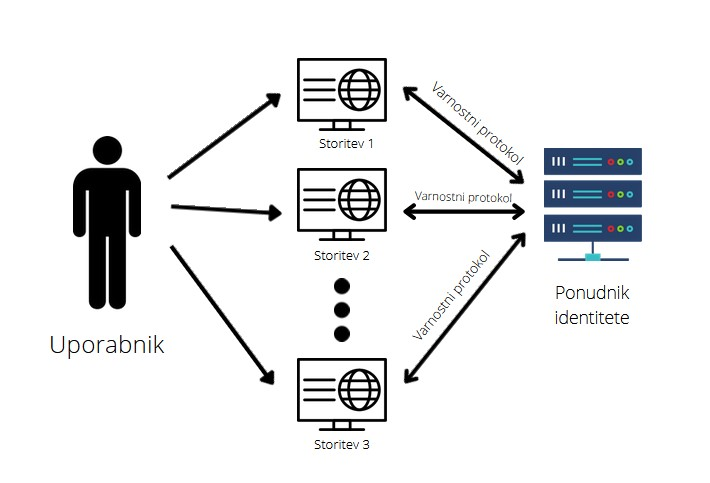
\includegraphics[scale=0.85]{diploma-FRI-vzorec_11maj2021/Prof_sistem.jpg}
\caption{Zasnova sistema}
\label{fig:zasnova sistema}
\end{figure}

\section{Uporabljene tehnologije}
\subsection{SAML}
\subsubsection{Kaj je SAML?}
SAML je akronim, ki se uporablja za Security Assertion Markup Language. Je odprt standard, ki se uporablja za preverjanje pristnosti. Njegova primarna vloga pri spletni varnosti je, da nam omogoča dostop do več spletnih aplikacij z enim parom uporabniškega imena in gesla za prijavo. Deluje tako, da posredujemo podatke za preverjanje pristnosti v določeni obliki med dvema strankama, običajno ponudnikom identitete (idP) in spletno aplikacijo. Spletne aplikacije na podlagi formata Extensible Markup Language (XML) uporabljajo SAML za prenos podatkov za preverjanje pristnosti.
\newline
Tehnološka industrija je ustvarila SAML za poenostavitev postopka preverjanja pristnosti, kjer so uporabniki morali dostopati do več neodvisnih spletnih aplikacij v različnih domenah. Ta lastnost je za nas glavna, ker ravno to je eden glavnih lastnosti, da ga bomo uporabili. Želimo, da če se želimo vpisati v e-mail račun lahko uporabimo enako uporabniško ime in geslo, kot pa če se želimo prijaviti v spletno učilnico. 

\subsubsection{Kako deluje SAML?}
SAML deluje tako, da izmenjuje uporabniške podatke, kot so prijave, stanje preverjanja pristnosti, identifikatorji in drugi ustrezni atributi med identiteto in ponudnikom storitev. Posledično se poenostavi in zavaruje postopek preverjanja pristnosti, saj se mora uporabnik prijaviti samo enkrat z enim samim parom uporabniškega imena in gesla za preverjanje pristnosti. Torej, ko uporabnik poskuša dostopati do spletnega mesta, ponudnik identitete posreduje preverjanje pristnosti SAML ponudniku storitev, ki nato odobri vnos uporabnika. Da bomo razumeli bolje, lahko uporabimo analogijo iz resničnega sveta.
\newline
Dober primer je letalska industrija. Preden se vkrcate na letalo, mora letalski prevoznik potrditi, da smo tisti, za katerega se predstavljamo, da zagotovi varnost drugih potnikov. Torej preverijo našo identiteto z neko obliko identifikacije s sliko, ki jo je izdal državni organ. Ko potrdijo, da se vaše ime na naši identiteti ujema z imenom na naši letalski vozovnici, nam nato dovolijo, da se vkrcamo na letalo.
\newline
Država je ponudnik identitete, letalska družba pa ponudnik storitev. Naša identifikacijska številka, ki jo je izdal državni organ, je trditev SAML. Ko zaprosimo za osebno izkaznico, moramo običajno izpolniti obrazec, se fotografirati in v nekaterih okoliščinah tudi oddati prstne odtise. Država (ponudnik storitev) nato te identifikacijske atribute shrani v svojo bazo podatkov in nam izda fizični ID, povezan z našo identiteto. V primeru letalske družbe, ko prispemo do izhoda, letalska družba (ponudnik storitev) preveri našo trditev ID (SAML). Letalska družba sprejme našo osebno izkaznico, saj vsebuje naše podatke, osebna izkaznica ali potni list pa se pregleda kot veljaven dokument. Po uspešni avtentikaciji nam letalska družba dovoli vkrcanje na letalo.

\subsubsection{Postopek avtentikacije z uporabom SAML-a}

SAML uporablja potek dela za preverjanje pristnosti, ki temelji na zahtevkih. Prvič, ko uporabnik poskuša dostopati do spletnega mesta, ponudnik storitev od ponudnika identitete zahteva, da preveri pristnost uporabnika. Nato ponudnik storitev uporabi trditev SAML, ki jo je izdal ponudnik identitete, da uporabniku odobri dostop. Ponazorimo potek dela s primerom.

\begin{itemize}
    \item Uporabnik odpre svoj brskalnik in se pomakne do spletne aplikacije ponudnika storitev, ki za preverjanje pristnosti uporablja ponudnika identitete.
    \item Spletna aplikacija se odzove z zahtevo SAML.
    \item Brskalnik posreduje zahtevo SAML ponudniku identitete.
    \item Ponudnik identitete razčleni zahtevo SAML.
    \item Če uporabnik ni overjen potem ponudnik identitete preveri pristnost uporabnika tako, da zahteva uporabniško ime in geslo ali kakšen drug faktor avtentikacije. Če je uporabnik že overjen, potem ponudnik identitete ta korak preskoči.
    \item Ponudnik identitete generira odgovor SAML in ga vrne v uporabnikov brskalnik.
    \item Brskalnik pošlje ustvarjen odgovor SAML spletni aplikaciji ponudnika storitev, ki ga preveri.
    \item Če je preverjanje uspešno, spletna aplikacija uporabniku odobri dostop.
\end{itemize}
\subsection{Wordpress}
Wordpress\cite{wordpress} je odprtokodni sistem za upravljanje vsebin. Funkcije vključujejo arhitekturo vtičnikov in sistem predlog, ki se v WordPressu imenujejo teme. WordPress je bil prvotno ustvarjen kot sistem za objavljanje spletnih dnevnikov.
\newline
Uporabljali ga bomo kot primer ponudnika storitev. Nekatere članice Univerze v Ljubljani ga uporabljajo za pisanje poročil znotraj razvojnih ekip in je popoln kandidat za ponudnika storitve. 
\subsection{Moodle}
Moodle\cite{Moodle} je brezplačen in odprtokoden sistem za upravljanje učenja, napisan v PHP in distribuiran pod GNU General Public License. Moodle se uporablja za učenje, izobraževanje na daljavo, učilnico in druge sheme spletnega učenja v šolah, na univerzah, na delovnih mestih in v drugih sektorjih.
\newline
Članice ga uporabljajo za gostovanje njihovih spletnih učilnic in je popoln kandidat za ponudnika storitev.
Moodle je primarno razvit v Linuxu z uporabo Apache, PostgreSQL/MySQL/MariaDB in PHP (včasih znan kot platforma LAMP). Običajno se tako izvaja tudi Moodle, čeprav obstajajo tudi druge možnosti, če so izpolnjene programske zahteve izdaje.
\subsection{MySQL}
MySQL je sistem za upravljanje s podatkovnimi bazami. MySQL je odprtokodna implementacija relacijske podatkovne baze, ki za delo s podatki uporablja jezik SQL.

MySQL deluje na principu odjemalec - strežnik, pri čemer lahko strežnik namestimo kot sistem, porazdeljen na več strežnikov. Obstaja veliko število odjemalcev, zbirk ukazov in programskih vmesnikov za dostop do podatkovne baze MySQL. Razvija ga Oracle Corporation. 

\subsection{PHP}
PHP\cite{php} (PHP Hypertext Preprocessor) je razširjen odprtokodni programski jezik, ki se uporablja za strežniške uporabe oziroma za razvoj dinamičnih spletnih vsebin. Lahko ga primerjamo z Microsoftovim sistemom ASP, VBScript in JScript, Sun Microsystemovim sistemom JSP in Java ter sistemom CGI in Perl.

Podoben je običajno strukturiranim programskim jezikom, najbolj jezikoma C in Perl, in najbolj izkušenim programerjem dovoljuje razvijanje zapletenih uporab brez dolgega učenja. 

\subsection{Nextcloud}

Nextcloud\cite{nextcloud} programska oprema je odprtokodna in brezplačna. Vsakdo jo lahko namesti in uporablja na svojih zasebnih strežniških napravah. 
Nextcloud je funkcionalno podoben Dropboxu, Office 365 ali Google Drive, če se uporablja z integriranimi rešitvami pisarniškega paketa Collabora Online ali OnlyOffice. Gostuje se lahko v oblaku ali na mestu uporabe. Razširljiv je od rešitev za domačo pisarno, ki temeljijo na poceni Raspberry Pi, pa vse do podatkovnih centrov polne velikosti, ki podpirajo milijone uporabnikov.

Nextcloud je popoln kandidat za integracijo v naš sistem kot ponudnik storitve. Članice ga uporabljajo za prenos in shranjevanje datotek v oblak. 

\subsection{Ponudnik identitete}
Preden lahko opišemo ponudnika identitete ga moramo izbrati. Na trgu je mnogo ponudnikov identitet, zato bomo definirali kriterije po katerem bomo ovrednotili potencialne ponudnike identitet in izbrali najbolj primernega. Kriteriji so naslednji:
\begin{itemize}
    \item odprtokodnost,
    \item brezplačnost,
    \item podpira protokol SAML2,
    \item podpira protokol LDAP,
    \item podpira dvofaktorsko avtentikacijo,
    \item podpira registracijo uporabnikov,
    \item število posodobitev kode na strani GitHub\cite{github} v zadnjem letu.
\end{itemize}

Ker bomo sistem postavili sami bomo potrebovali celoten dostop do ozadja, zato je ključnega pomena, da je program odprtokoden. V sklopu diplomskega dela nimamo proračuna, zato mora biti sama nastavitev brezplačna. Ponudnik identitete mora podpirati protokol SAML2, ker je ključen za implementacijo federacijske avtentikacije. Prav tako mora podpirati protokol LDAP, saj so nekatere storitve v sistemu Univerze v Ljubljani dosegljive samo preko tega protokola kot npr. Eduroam. Podpirati mora dvofaktorsko avtentikacijo, ki nam bo služila kot sistem ponastavitve gesla in registracijo uporabnikov, če se za to odločimo. Zadnji kriterij nam bo služil kot približna ocena aktivnosti uporabnikov in razvijalcev na projektu. Število sprememb se bo merilo med obdobjem od 8.8.2021 do 24.7.2022. Želimo, da se ponudnik identitete aktivno razvija in ima aktivno bazo uporabnikov in razvijalcev.

\subsubsection{Authentik}
\begin{itemize}
    \item odprtokodnost: je odprtokoden,
    \item brezplačnost: je brezplačen,
    \item podpira protokol SAML2: ga podpira,
    \item podpira protokol LDAP: ga podpira,
    \item podpira dvofaktorsko avtentikacijo: jo podpira,
    \item podpira registracijo uporabnikov: jo podpira,
    \item število posodobitev kode na strani GitHub v zadnjem letu: 3333\cite{AuthentikGit},
\end{itemize}

\subsubsection{Keycloak}
\begin{itemize}
    \item odprtokodnost: je odprtokoden,
    \item brezplačnost: je brezplačen,
    \item podpira protokol SAML2: ga podpira,
    \item podpira protokol LDAP: ga podpira,
    \item podpira dvofaktorsko avtentikacijo: jo podpira,
    \item podpira registracijo uporabnikov: jo podpira,
    \item število posodobitev kode na strani GitHub v zadnjem letu: 1164\cite{KeycloakGit},
\end{itemize}
\subsubsection{Authellia}
\begin{itemize}
    \item odprtokodnost: je odprtokoden,
    \item brezplačnost: je brezplačen,
    \item podpira protokol SAML2: ga ne podpira,
    \item podpira protokol LDAP: ga podpira,
    \item podpira dvofaktorsko avtentikacijo: jo podpira,
    \item podpira registracijo uporabnikov: jo ne podpira,
    \item število posodobitev kode na strani GitHub v zadnjem letu: 983\cite{AuthelliaGit},
\end{itemize}
\subsubsection{Odločitev za ponudnika identitete}
Za ponudnika identete smo izbrali Authentik. Od predstavljenih možnosti je najbolj primeren. Ustreza vsem potrebnim kriterijem in ima največje število posodobitev kode na spletni strani GitHub. 
\subsection{Authentik}
Authentik\cite{AuthentikLink} je odprtokoden ponudnik identitete, osredotočen na prilagodljivost in vsestranskost. Authentik lahko uporabimo v obstoječem okolju, da dodamo podporo za nove protokole, implementiramo prijavo, obnovitev itd. Preverjanje pristnosti izvajamo po meri ali pa z logiko nadzora dostopa s kodo Python.
\newline
Uspešna namestitev Authentika ima par zahtev.
Potrebovali bomo operacijski sistem Linux z vsaj dvema jedroma in vsaj 2GB RAM-a. Poleg tega bomo potrebovali docker ter docker-compose. 

\subsection{Docker}
Docker\cite{dockerLink} je odprtokodna tehnologija kontejnerizacije za gradnjo in posodabljanje naših aplikacij.
Docker deluje kot aplikacija odjemalec-strežnik z:
\begin{itemize}
    \item strežnikom z dolgo delujočim demonskim procesom dockerd,
    \item API (Application Programming Interface), ki določajo vmesnike, ki jih lahko programi uporabljajo za pogovor in ukazovanje demonu Docker,
    \item Docker odjemalca vmesnika ukazne vrstice CLI (Command Line Interface).
\end{itemize}
CLI uporablja API-je Docker za nadzor ali interakcijo z demonom Docker prek skriptiranja ali neposrednih ukazov CLI. Številne druge aplikacije Docker uporabljajo osnovni API in CLI. Demon ustvarja in upravlja objekte Docker, kot so slike, vsebniki, omrežja in nosilci.

\subsection{Docker Compose}
\label{Docker}
Docker Compose\cite{dockerComposeLink} je orodje za definiranje in izvajanje aplikacij Docker z več kontejnerji. Z možnostjo Compose uporabimo datoteko YAML za konfiguriranje storitev aplikacij. Nato z enim ukazom ustvarimo in zaženemo vse storitve iz konfiguracij.

\chapter{Rešitev}
\section{Upravljanje s študentskimi identitetami}
Ko je kandidat sprejet na študijsko smer, se zanj generira študentska identiteta. Študetnska identiteta se potrebuje, da študent lahko dostopa do e-učilnic, e-mail naslovov, si z njo izposoja gradivo v knjižnjici itd. Ob koncu študija konča, se identiteta deaktivira in postane neaktivna. 
Za boljše razumevanje bomo definirali naslednje vloge:
\begin{itemize}
    \item \textbf{kandidat} je vsaka oseba, ki ima možnost, da se na študij vpiše in se je na enega izmed študijskih programov tudi vpisal;
    \item \textbf{študent} je kandidat, ki je bil uspešno vpisan na študijski program;
    \item \textbf{bivši kandidat} je kandidat, ki mu je bil vpis na študijsko smer zavrnjen oz. če kandidat svoj vpis zavrne;
    \item \textbf{bivši študent} je študent, ki je bil izključen, se je izpisal, nima pogojev za ponavljanje letnika ali študij dokončal.
\end{itemize}
Vsaka oseba ima možnost, da se vpiše na študij. Na tem mestu bomo to osebo označili kot \emph{kandidat}. \emph{Kandidat}  je vsak, ki se je vpisal na enega izmed študijskih programov. V tem koraku ima postopek dva možna izida. Prva možnost je, da je \emph{kandidat} sprejet in je uspešno vpisan na študijski program. S tem pridobi vlogo \emph{študenta}. V nasprotnem primeru (je zavrnjen) in pridobi vlogo \emph{bivšega kandidata}. Do enakega izida pride v primeru, če \emph{kandidat} svoj vpis prekliče. \newline
Ko je \emph{kandidat} vpisan, prestopi v vlogo \emph{študenta}, torej se nahaja v aktivnem procesu študiranja. Med študijem je \emph{študent} lahko izključen ali pa se s študija prostovoljno izpiše. Če pride do tega, postane \emph{bivši študent}. Če je uspešen, torej če letnik uspešno zaključi oz. diplomira, se mu prav tako dodeli vloga \emph{bivši študent}, saj je študij zaključil. Če ni diplomiral, obstaja možnost, da je opravil letnik oz. mora letnik ponavljati. V tem primeru ni spremembe stanja (ostane mu vloga \emph{študent}). Če študent ne izpolnjuje pogojev za ponavljanje letnika oz. za vpis v višji letnik, se mu študij prekine, zato dobi vlogo \emph{bivši študent}.
Vsak, ki je kadarkoli imel vlogo študenta (torej vse osebe z vlogami \emph{študent} oz. \emph{bivši študent}) ima oz. je imel na univerzi svojo identiteto. 
Celoten postopek viden na sliki \ref{fig:student}
\begin{figure}[H]
    \centering
    \includegraphics[width=0.8\textwidth]{diploma-FRI-vzorec_11maj2021/ID MANAGEMENT ZA ŠTUDENTE.png}
    \caption{\label{fig:student} Upravljanje s študentskimi identitetami}
\end{figure}
Naša naloga je, da vzpostavimo sistem, kjer bo vsaka oseba z vlogo \emph{študent} imel dostop do večjega števila storitev z samo enim parom uporabniškega imena in gesla. 
\section{Namestitev Docker in Docker Compose}
Za namestitev docker na sistemu Ubuntu lahko sledimo uradni spletni strani \cite{DockerLink}, ki nas vodi skozi proces. Najprej bomo odstranili morebitne stare verzije. V primeru da le-te niso prisotne, ukaz ne bo imel negativnih posledic.

 \texttt{ \$ sudo apt-get remove docker docker-engine docker.io containerd runc}

 Nato lahko naložimo Docker. Obstaja več možnih načinov. Mi bomo uporabili curl.
 Ukaz curl je orodje za prenos datotek ali podatkov s strežnika ali na strežnik z uporabo FTP, HTTP, HTTPS, SCP, SFTP, SMB in drugih podprtih protokolov v sistemih Linux ali Unixu. Če curl ni nameščen na sistem, ga moramo naložiti z uporabo apt oz. apt-get ukaza. To lahko naredimo preprosto, z naslednjimi ukazi.
 
\begin{lstlisting}[language=bash]
$ sudo apt update
$ sudo apt upgrade
$ sudo apt install curl
\end{lstlisting}

Sedaj imamo zadoščene vse predpogoje za namestitev dockerja. To storimo z naslednjimi ukazi.

\begin{lstlisting}[language=bash]
$  curl -fsSL https://get.docker.com -o get-docker.sh
$  sudo sh get-docker.sh
\end{lstlisting}

Od zahtev za namestitev Authentika nam sedaj manjka samo še Docker Compose. Navodila za njegovo namestitev najdemo na spletni strani \cite{DockerCompose}. 
Tudi Docker Compose bomo namestili z uporabo prej nameščenega ukaza curl.


\begin{lstlisting}[language=bash]
$ curl -SL https://github.com/docker/compose/releases/
download/v2.5.0/docker-compose-linux-x86_64 -o /
usr/local/bin/docker-compose

$   sudo chmod +x /usr/local/bin/docker-compose
\end{lstlisting}

Namestitev nam je uspela, če se nam izpiše verzija Docker Compose-a, ko izvedemo naslednji ukaz.

\begin{lstlisting}[language=bash]
$  docker-compose --version
\end{lstlisting}
\section{Namestitev Authentika}

Na tej točki imamo zadoščene vse predhodne zahteve. Začnemo lahko z namestitvijo ponudnika identitet. Kot omenjeno v poglavju \ref{Docker}, bomo za konfiguracijo sistema uporabili datoteko YAML. Datoteko YAML lahko dobimo na uradni spletni strani Authentika\cite{AuthentikYAML} in jo postavimo v direktorij, kjer želimo imeti naš projekt. 

Docker Compose projekt vsebuje naslednje kontejnerje:

\begin{itemize}
    \item Server. To je zaledna storitev, ki izvaja vso logiko, izvaja API in dejanski del SSO. Prav tako poganja sprednji del, gosti datoteke JS/CSS in služi tudi datotekam, ki smo jih naložili za ikone itd.
    \item Worker. Ta kontejner izvaja opravila v ozadju, vse, kar lahko vidite na strani Sistemska opravila v sprednjem delu.
    \item Redis in PostgreSQL. Predpomnilnik in baza podatkov.
\end{itemize}

Ker je to sveža namestitev Authentika, moramo še zgenerirati geslo. V ukaznem pozivu se premaknemo v direktorij, kamor smo shranili prej omenjeno YAML datoteko. Sedaj napišemo naslednje ukaze.

\begin{lstlisting}[language=bash]
$  sudo apt-get install -y pwgen
echo "PG_PASS=$(pwgen -s 40 1)" >> .env
echo "AUTHENTIK_SECRET_KEY=$(pwgen -s 50 1)" >> .env
\end{lstlisting}

Zaradi omejitve PostgreSQL so podprta gesla samo do 99 znakov. Več o tem si lahko preberete na uradni strani od PostgreSQL \cite{PostgreSQL}. Kljub temu bo v našem primeru zadostovalo. \newline

V .env datoteki v našem direktoriju se trenutno nahaja naše geslo. Poleg tega lahko v .env datoteko dodamo dve vrstici kode, da bo Authentik tekel na bolj prepoznavnih vratih 80/443. 

\begin{lstlisting}[language=bash]
AUTHENTIK_PORT_HTTP=80
AUTHENTIK_PORT_HTTPS=443
\end{lstlisting}

Sedaj poženemo naslednji ukaz, da se spremembe uveljavijo. 

\begin{lstlisting}[language=bash]
$ sudo docker-compose up -d
\end{lstlisting}

Za dokončanje namestitve moramo izvesti še dva ukaza, ki bosta sistem tudi zagnala.

\begin{lstlisting}[language=bash]
$ sudo docker-compose pull
$ sudo docker-compose up -d
\end{lstlisting}

Naš ponudnik identitete je postavljen. Da začnemo z upravljanjem našega ponudnika identitet, navigiramo na naslov: 
\newline
\texttt{https://<serverIP>/if/flow/initial-setup/} 
\newline
\texttt{<serverIP>} moramo zamenjati z IP naslovom našega Ubuntu serverja. To lahko naredimo tako, da v ukazni poziv vpišemo naslednji ukaz:
\begin{lstlisting}[language=bash]
 $ ip addr show
\end{lstlisting}

Iz vrnjenjih podatkov razberemo naš IP naslov, ter z njim zamenjamo značko \texttt{<serverIP>}. Ta naslov nas preusmeri na stran, kjer moramo določiti geslo za administratorja. 

\section{Namestitev Wordpressa}
Za ponudnika storitev bomo gostili spletno stran Wordpress. Uporabniki se bodo lahko prijavili v spletno stran, kjer bodo lahko urejali izgled, pisali objave, upravljali nastavitve ipd. 
Neprijavljeni uporabniki bodo lahko samo brali objave. 
\newline
Namestitev Wordpressa bo lažja. Že pred pisanjem diplomskega dela sem imel v lasti svojo domeno, ki jo gostim preko hostinger.com in je dostopna na \href{www.davidkonc.xyz}{www.davidkonc.xyz} (dostopano 30.05.2022). 
Spletna stran je uporabniku prijazna, ima namreč veliko pripomočkov, ki nam bodo delo olajšali.
Preko uporabniškega vmesnika lahko registriramo domeno. Za ime domene sem izbral davidkonc.xyz. Le-to sem uporabljal za življenjepis, pred pisanjem mojega diplomskega dela. 
Po uspešni registraciji domene lahko kliknemo na gumb "Manage", ki nas usmeri na meni, ki upravlja z našo spletno stranjo..

Na upravljalni plošči naše spletene strani lahko vidimo gumb "Install Wordpress". Ta omogoča samodejno namestitev Wordpress vmesnika na našo spletno stran. Sedaj je na naši spletni strani (\href{www.davidkonc.xyz}{www.davidkonc.xyz}) viden osnoven Wordpress blog.

\section{Namestitev Moodla}
Za namestitev bomo uporabili trik. V že obstoječo mapo, kjer imamo trenutno vse datoteke, ki nam služijo za delovanje Wordpressa bomo premaknili vse potrebne datoteke, ki so potrebne za delovanje Moodla. Te datoteke lahko najdemo na naslovu \href{https://download.moodle.org/releases/latest/}{https://download.moodle.org/releases/latest/}. Naša storitev bo tako dostopna na enakem spletnem naslovu, samo v poddirektoriju moodle (dostopno na \href{https://davidkonc.xyz/moodle/}{https://davidkonc.xyz/moodle/}).
\newline
Za pravilno delovanje Moodla bomo potreblovali še MySQL databazo. To bomo storili preko uporabniškega vmesnika na našem gostitelju spletne strani Hostinger. Vse kar od nas potrebuje so naslednji podatki:
\begin{itemize}
    \item ime databaze,
    \item uporabniško ime za uporabnika baze,
    \item geslo za uporabnika baze.
\end{itemize}
Te podatke si zapišemo, ker jih bomo potrebovali pri namestitvi v naslednjem koraku. 
\newline
Sedaj imamo vse pipravljeno, da začnemo z namestitvijo. Če gremo na domačo spletno stran \href{www.davidkonc.xyz/moodle/index.php}{www.davidkonc.xyz/moodle/index.php} nas bo pri prvem obisku te strani pričakal čarovnik za namestitev. 

V prvem meniju izberemo jezik, v katerem želimo imeti naš Moodle. Izberemo slovenščino. V drugem meniju samo potrdimo pot do naših datotek. V tretjem meniju vnesemo podatke o databazi, ki smo jo kreirali za ta namen. Uporabimo podatke, ki smo jih izbrali. Naslednja dva menija imamo samo možnost potrditve. Eden nas sprašuje, če se strinjamo s pogoji uporabe in naslednji nas sprašuje kateri dodatki se bodo namestili na spletno stran. Po tem sledi samo še zadnji meni, kjer nastavimo uporabniško ime in geslo za administratorskega uporabnika. S temi podatki se sedaj lahko prijavimo v Moodle kot administrator. 

\section{Namestitev Nextclouda}

Namestitev Nextclouda bo podobna namestitvi Moodla. Potrebne datoteke lahko najdemo na \href{https://nextcloud.com/install/}{https://nextcloud.com/install/}. Te datoteke premaknemo v naš direktorij pri spletnem gostitelju. Ponovno ustvarimo MySQL databazo s podatki o imenu databaze, uporabniškem imenu in geslom. Te podatke si zapišemo, ker jih bomo potrebovali v naslednjem koraku.
\newline
Navigiramo na spletno mesto, kjer smo postavili datoteke (v našem primeru je to \href{www.davidkonc.website/index.php}{www.davidkonc.website/index.php}). Ponovno nas pričaka čarovnik za namestitev, ki od nas zahteva naslednje podatke:
\begin{itemize}
    \item uporabniško ime za administratorski račun,
    \item geslo za administratorski račun,
    \item ime uporabnika MySQL databaze,
    \item geslo uporabnika MySQL databaze,
    \item ime MySQL databaze.
\end{itemize}

Ko priskrbimo oz. izberemo vse potrebne podatke, se namestitev sama konča. Z izbranim uporabniškim imenom in geslom imamo dostop do administratorskega uporabnika.

\chapter{Dodajanje storitev iz federacije}

Sedaj imamo nameščene oz. izbrane naslednje komponente v našem sistemu:
\begin{itemize}
    \item ponudnik identitete (Authentik),
    \item ponudnik storitve (Wordpress),
    \item ponudnik storitve (Moodle),
    \item ponudnik storitve (Nextcloud),
\end{itemize}
Naš naslednji korak je, da vsako izmed ponudnikov storitev povežemo z našim ponudnikom identitete, tako da bomo lahko do vsake storitve dostopali z enakim uporabniškim imenom in geslom. To bomo dosegli z uporabo SAML avtentikacije pri vsakem ponudniku storitve. 

\section{Povezava Wordpress-Authentik}
\label{authwp}

Ker imamo za ponudnika storitev Wordpress, se lahko poslužimo enega izmed mnogih vtičnikov, ki bo naredil SAML implementacijo za nas enostavno.  

V zavihku Plugins (vtičniki) izberemo možnost Add new (dodaj novo). Če v okno za iskanje vnesemo besedo ''SAML'', se nam prikaže vtičnik  ''SAML Single Sign On - SAML SSO Login'', ki ga je naredilo podjetje miniOrange\cite{miniOrange}. 
\newline
Ko ga namestimo, se nam prikaže nov meni z imenom ''miniOrange SAML 2.0 SSO''. Ta meni in meni v Authentiku bomo sedaj uporabili, da vzpostavimo avtentikacijo. 
\newline
Najprej pojdimo v Authentik meni, da najprej naredimo aplikacijo na ponudniku identitet. Navigiramo na IP-naslov našega ponudnika in se vpišemo z uporabniškim imenom administratorja, ki smo ga nastavili, ko smo nameščali Authentik. Ko se prijavimo, lahko vidimo, da še nimamo aktivnih aplikacij. Navigiramo na "Admin interface" (skrbniški vmesnik), kjer lahko sedaj na levi strani v meniju vidimo vse možnosti.

Izberemo možnost Applications in Create, tukaj moramo pa sedaj specificirati vse potrebno, za uspešno povezavo. Tu je pomembno okno Provider (ponudnik), ki ga moramo tudi narediti. To bo naša implementacija SAML-a.Lahko kar kliknemo gumb Create provider (naredi ponudnika) in izberemo možnost ''SAML Provider''. 
Od nas se bodo zahtevali naslednji podatki in vnesli bomo naslednje:
\begin{itemize}
    \item Name (ime): Wordpress (izberemo sami).
    \item Authorization flow: default-provider-authorization-explicit-consent
    \item ACS URL: ta podatek pridobimo na strani vtičnika na naši Wordpress strani - v našem primeru je to: https://davidkonc.xyz/
    \item Issuer: ta podatek pridobimo na strani vtičnika na naši Wordpress strani - v našem primeru je to: https://davidkonc.xyz/wp-content/plugins/miniorange-saml-20-single-sign-on/
    \item Service Provider Binding:  Post
\end{itemize}

Ko imamo ustvarjeneva ponudnika (Provider) v Authentiku, lahko dokončamo ustvarjanje aplikacije. Izpolniti moramo naslednje možnosti:
\begin{itemize}
    \item Name (ime): Wordpress (izberemo sami).
    \item Slug: Wordpress (izberemo sami).
    \item Provider: Wordpress (ime od pravkar ustvarjenega ponudnika).
    \item Policy engline mode: ANY, any policy must match to grant access (privzeta vrednost). 
\end{itemize}

Sedaj smo na strani Authentika opravili. Konfigurirajmmo še vtičnik v Wordpressu. V meniju vtičnika izberemo ''Service Provider Setup'' in izberemo možnost ''Upload IDP Metadata''. Tukaj moramo sedaj vnesti XML datoteko z metapodatki od našega ponudnika identitet. To lahko dobimo pri našem ponudniku identitet v zavihku ''Provider'', kjer izberemo ponudnika, ki smo ga mi kreirali in ga izberemo. Na dnu strani se nam pojavi veliko okno z vsemi metapodatki. To lahko prenesemo, da potem naložimo v vtičnik v Wordpressu. 

\begin{figure}[H]
\hspace{-4cm}
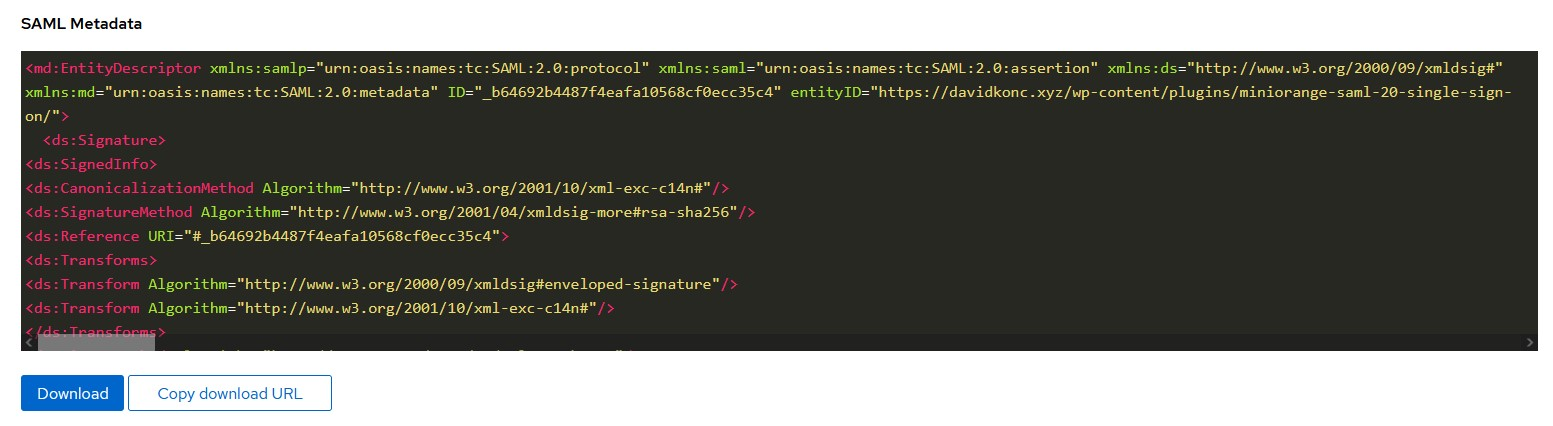
\includegraphics[scale=0.5]{diploma-FRI-vzorec_11maj2021/SAMLMetadata.jpg}
\caption{Metapodatki v Authentiku}
\label{fig}
\end{figure}

S povezavo smo s tem zaključili. V prijavnem meniju lahko sedaj vidimo možnost prijave z Authentikom, ki nas preusmeri na spletno stran Authentika, če ga pritisnemo. 

\section{Povezava Moodle-Authentik}

Za povezavo Moodla z Authentikom bomo prav tako uporabili vtičnik, ki ga Moodle podpira. Preden storimo to, pa pripravimo vse potrebno v Authentiku. Ustvarimo novega ponudnika. Izberemo oz. določimo naslednje podatke:

\begin{itemize}
    \item Name (ime): Moodle (izberemo sami).
    \item Authorization flow: default-provider-authorization-explicit-consent
    \item ACS URL: https://davidkonc.xyz/moodle/auth/saml2/sp/saml2-acs.php/davidkonc.xyz
    \item Issuer: https://davidkonc.xyz/moodle/auth/saml2/sp/metadata.php
    \item Service Provider Binding:  Post
\end{itemize}

Nato ustvarimo aplikacijo z naslednjimi podatki:
\begin{itemize}
    \item Name (ime): Moodle (izberemo sami).
    \item Slug: moodle (izberemo sami).
    \item Provider: Moodle (ime od pravkar ustvarjenega ponudnika).
    \item Policy engline mode: ANY, any policy must match to grant access (privzeta vrednost). 
\end{itemize}

Na strani Authentika imamo sedaj vse pripravljeno. Podobno storimo pri Moodlu. 

Vtičnik lahko prenesmo na spletni strani \href{https://moodle.org/plugins/}{https://moodle.org/plugins/}. Ime našega vtičnika je ''SAML2 Single sign on''. V Moodle meniju, gremo v meni "Plugins", kamor naložimo prenesen vtičnik. 
Navigiramo do nastavitev pravkar nameščenega vtičnika. Tu lahko vidimo veliko možnosti, ampak nas bodo zanimale samo naslednje, ki jih primerno nastavimo:
\begin{itemize}
    \item IdP metadata xml OR public xml URL: metadato dobimo v Authentiku, v našem pravkar ustvarjenem podnudniku.
    \item IdP label override: Authentik! (izberemo, kaj bo pisalo na gumbu za prijavo).
    \item Allow create: Yes. (možnost omogoči ustvarjanje uporabnikov).
\end{itemize}
S povezovanjem smo sedaj zaključili. V meniju za prijavo lahko sedaj vidimo možnost za prijavo z Authentikom.

\section{Povezava Nextcloud-Authentik}
V Authentiku ponovno kreiramo ponudnika za naslednjimi nastavitvami:
\begin{itemize}
    \item Name (ime): nextcloud-saml (izberemo sami).
    \item Authorization flow: default-provider-authorization-explicit-consent 
    \item ACS URL: https://davidkonc.website/index.php/apps/user\_saml/saml/acs
    \item Issuer: http://vmi868001.contaboserver.net/ (domena našega Authentika).
    \item Service Provider Binding:  Post
    \item Signing Certificate: authentik Self-signed Certificate
\end{itemize}
Pri ustvaritvi aplikacije uporabimo naslednje nastavitve:

\begin{itemize}
    \item Name (ime): Nextcloud (izberemo sami).
    \item Slug: nextcloud (izberemo sami).
    \item Provider: nextcloud\_saml (ime od pravkar ustvarjenega ponudnika).
    \item Policy engline mode: ANY, any policy must match to grant access (privzeta vrednost). 
\end{itemize}

Poleg tega bomo za uspešno povezavo potrebovali še certifikat od Authentika, ki ga lahko pridobimo v zavihku ''Certificates''. Sedaj pa uredimo še na strani Nextclouda.

V administratorskem okolju navigiramo v zavihek ''Orodja'', kjer lahko namestimo vtičnik ''Overitev SSO in SAML''. Nato navigiramo v nastavitve tega vtičnika. Tukaj nastavimo naslednje nastavitve:

\begin{itemize}
    \item Dovoli uporabo več uporabniških računov: DA,
    \item Izbirno prikazno ime ponudnika istovetnosti: authentik,
    \item Dovolilo IdP (zapisano kot naslov URI): http://vmi868001.contaboserver.net,
    \item Ciljni naslov URL za IdP, kamor bo ponudnik storitev poslal sporočilo o zahtevi overtive: http://vmi868001.contaboserver.net/application/saml
    /nextcloud\_meta/sso/binding/redirect/
    \item Ciljni naslov URL za IdP, kamor bo ponudnik storitev poslal zahtevo SLO:http://vmi868001.contaboserver.net/
    if/session-end/nextcloud\_meta/
    \item Javno potrdilo X.509 IdP: Priskrbeni certifikat od Authentika. 
    \item Atribut za preslikavo prikaznega imena: http://schemas.xmlsoap.org/ws/2005/05/
    identity/claims/name
    \item Atribut za preslikavo elektronskega naslova: http://schemas.xmlsoap.org/ws/
    2005/05/identity/claims/emailaddress
    \item Atribut za preslikavo uporabniških skupin: http://schemas.xmlsoap.org/claims/Group
\end{itemize}

S povezovanjem smo sedaj zaključili. V meniju za prijavo lahko sedaj vidimo možnost za prijavo z Authentikom.


\section{Test konfiguracije}

Z implementacijo smo sedaj zaključili. Preverimo, če sedaj vse deluje kot mora. 
To bomo naredili na naslednji način:
\begin{itemize}
    \item V direktoriju uporabnikov v Authentiku bomo ustvarili novega uporabnika, ki bo predstavljal uporabniški račun, ki bi ga imel študent.
    \item Navigirali bomo na prijavno stran od vsakega ponudnika storitev (Wordpress, Moodle, Nextcloud), ter se poskusili prijaviti z uporabniškim imenom in geslom od novo ustvarjenega uporabnika. Če je prijava uspešna, implementacija deluje. 
\end{itemize}

V Authentiku navigirajmo v direktorij ''Users'' (uporabniki), kjer lahko ustvarimo novega uporabnika s pritiskom gumba ''Create'' (ustvari). Vse kar potrebujemo je uporabniško ime, ki si ga izberemo, v tem primeru bomo izbrali ime ''student''. Ko smo ga ustvarili, kliknemo na novo ustvarjenega uporabnika, ter izberemo možnost ''Set password'' (nastavi geslo). Izberemo geslo.  

\subsubsection{Prijava v Wordpress}
Navigirajmo na prijavno stran od Wordpressa, kjer sedaj lahko opazimo gumb ''Login with Authentik''. To bo sedaj naša izbira prijave. Ko pritisnemo ta gumb nas preusmeri na stran Authentika, kjer sedaj vpišemo uporabniško ime in geslo novega uporabnika. Če je prijava uspešna, lahko sedaj vidimo administratorski pogled z vsemi možnostmi v meniju. 

\subsubsection{Prijava v Moodle}
Navigirajmo na prijavno stran od Moodla, kjer sedaj lahko opazimo gumb ''Authentik!''. To bo sedaj naša izbira prijave. Ko pritisnemo ta gumb nas preusmeri na stran Authentika, kjer sedaj vpišemo uporabniško ime in geslo novega uporabnika. Če je prijava uspešna, nas preusmeri v meni, kjer moramo nastaviti ime, priimek in e-poštni naslov. Ko storimo to, imamo dostop do učilnice. 

\subsubsection{Prijava v Nextcloud}
Navigirajmo na prijavno stran od Nextclouda, kjer sedaj lahko opazimo gumb ''authentik''. To bo sedaj naša izbira prijave. Ko pritisnemo ta gumb nas preusmeri na stran Authentika, kjer sedaj vpišemo uporabniško ime in geslo novega uporabnika. Če je prijava uspešna, nas preusmeri v Nextcloud z že ustvarjenim uporabnikom, kjer imamo sedaj poln dostop. 

\chapter{Zaključek}

V tem diplomskem delu smo razvili novo avtentikacijsko rešitev za potencialno uporabo na Univerzi v Ljubljani. Vzpostavili smo ponudnika identitete Authentik, ki je odprtokoden in sicer na naš Ubuntu Serverju. Vzpostavili smo ponudnike storitev, ki bodo potrebovali avtentikacijo. Za to nalogo smo izbrali Wordpress, Moodle ter Nextcloud zaradi vnaprej ponujenih vtičnikov, ki so nam olajšali delo. Za povezavo med njimi pa smo izbrali protokol SAML, ki podpira federacijsko avtentikacijo, da lahko uporabnikom omogočimo preprostejšo prijavo na več storitev. 
\newline
Sestava sistema nam je uspela in smo se uspešno prijavili v vse ponudnike storitev s tem, da smo se avtenticirali pri našem ponudniku identitete (Authentik). 
\newline
Ampak žal naša rešitev ni brez pomankljivosti. Najbolj pogosti dve pomanjkljivosti nista odpravljeni s federacijsko avtentikacijo. To so notrajnje grožnje in kraja identitete. Biti moramo popolnoma prepričani v zanesljivost uporabnikov v omrežju in imeti protokole za preverjanje pristnosti zasnovane tako, da zagotovijo, da je vsak uporabnik tisti, za katerega trdi, da je. Izobraževanje uporabnikov je potrebno za zmanjšanje tveganja človeške napake, saj lahko en sam ogrožen par federacijskih poverilnic hekerjem omogoči dostop do več aplikacij in omogoči hitro širjenje kršitve po omrežju.
Nepravilna oskrba, ki vodi do prekoračitve privilegijev, lahko pusti odprta vrata za kršitve. Uporabnikova združena identiteta bi morala omogočati le raven dostopa, ki je potrebna za njegovo ali njeno delo in vsak začasni dostop, potreben za kratkoročne projekte, je treba preklicati takoj, ko ni več potreben. Avtomatizirane rešitve za odobritev in preklic dostopa postajajo vse pogostejša.
\newline
Našo rešitev bi lahko nadgradili tako, da bi vzpostavili sistem skupin, kjer bi vsakega uporabnika uvrstili v primerno skupino in potem prirejali pravice skupinam. To bi bil najlažji sistem vzdrževanja pravic uporabnikom, ker jim bi bilo potrebno samo določiti vlogo v sistemu. Tako bi potem uporabniki imeli dostop do aplikacij, ki so vezani na to vlogo. 
\newline
Prav tako bi lahko rešitev nadgradili, da bo uporabili več varnostnih protokolov, kot so npr. LDAP (Lightweight Directory Access Protocol) oz. OIDC (OpenID Connect). Vse aplikacije v sistemu Univerze v Ljubljani ne uporabljajo SAML avtentikacije, ampak nekatere uporabljajo tudi druge (npr. Eduroam uporablja LDAP za avtentikacijo). 
\newline
Za zaključek bi dodali, da čeprav naša rešitev ni popolna, odpravlja glavne pomanjkljivosti avtentikacije, ki bi nam olajšale prijavo, s tem pa bi bolje zavarovali sistem. 



\cleardoublepage
%\addcontentsline{toc}{chapter}{Literatura}

\printbibliography[heading=bibintoc,type=article,title={Članki v revijah}]

\printbibliography[heading=bibintoc,type=inproceedings,title={Članki v zbornikih}]

\printbibliography[heading=bibintoc,type=incollection,title={Poglavja v knjigah}]

\printbibliography[heading=bibintoc,title={Celotna literatura}]


\end{document}

